\documentclass[10pt,twocolumn,letterpaper]{article}
%% Welcome to Overleaf!
%% If this is your first time using LaTeX, it might be worth going through this brief presentation:
%% https://www.overleaf.com/latex/learn/free-online-introduction-to-latex-part-1

%% Researchers have been using LaTeX for decades to typeset their papers, producing beautiful, crisp documents in the process. By learning LaTeX, you are effectively following in their footsteps, and learning a highly valuable skill!

%% The \usepackage commands below can be thought of as analogous to importing libraries into Python, for instance. We've pre-formatted this for you, so you can skip right ahead to the title below.

%% Language and font encodings
\usepackage[english]{babel}
\usepackage[utf8x]{inputenc}
\usepackage[T1]{fontenc}
\usepackage{amsmath}

%% Sets page size and margins
\usepackage[a4paper,top=3cm,bottom=2cm,left=3cm,right=3cm,marginparwidth=1.75cm]{geometry}

%% Useful packages
\usepackage{amsmath}
\usepackage{graphicx}
\usepackage[colorinlistoftodos]{todonotes}
\usepackage[colorlinks=true, allcolors=blue]{hyperref}
\usepackage{natbib}
\bibliographystyle{unsrt}
%% Title
\title{
		\usefont{OT1}{bch}{b}{n}
		\normalfont \normalsize \textsc{SPH 4U1} \\ [10pt]
		\huge Atwood Machine Lab Report \\
}
\selectlanguage{english}
\usepackage{authblk}
\usepackage{amssymb}
\author[1]{Hanz Nathan Po}

\begin{document}
\maketitle

\section{Objective}
The objective of this lab is to explore the effects of Newton’s laws by exploring the motion in various parts of Atwood’s pulley machine.

\section{Introduction}
An Atwood machine, also known as Atwood’s machine, is a device first introduced by George Atwood. He was an English mathematician who wanted to explore constant acceleration following Newton’s laws of motion. An Atwood machine typically consists of a string that can move freely along a pulley. The string is tied to two masses, \(m_{1}\) and \(m_{2}\). Both of the masses experience a constant acceleration, dependent on the masses. When \(m_{1} = m_{2}\), acceleration is zero because the machine is in a state of equilibrium. 

Exploring the motions of the masses in an Atwood machine requires an understanding of various kinematics concepts as well as Newton’s laws of motion. Kinematics refers to the motion of an object without considering the forces that cause them to move. Using Newton’s laws of motion, it is possible to relate the motion of the object with the forces acting upon it. There exists one common kinematics formula provides distance given the acceleration, change in time, and initial velocity. 

\begin{equation}
    \overrightarrow{\Delta d}=\overrightarrow{v_{i}}\Delta t+\frac{1}{2}\overrightarrow{a}\Delta t^2
\end{equation}

Rearranging this equation and assuming that the initial velocity is zero, we can solve for acceleration. This will be especially useful in the lab because the objective is to calculate the acceleration of the masses.

\begin{equation}
    a=\frac{2\Delta d}{\Delta t^2}
\end{equation}

In the rearranged equation, \(a\) refers to the acceleration in the system. The magnitude of this value is equal to both masses in the system. Since the initial velocity is zero, we can remove a term from the rearranged equation. The \(\Delta d\) represents the change in displacement, of which the magnitude is also equal to both masses. Finally, the \(\Delta t\) represents the change in time.

When observing the effects of forces on an Atwood machine, it is important to take note of Newton's Laws. Isaac Newton was an English mathematician, physicist, and astronomer who defined three laws of motion. The most important one when calculating the effects of forces on an Atwood machine is the second law of motion, which can be written as 

\begin{equation}
    F = ma
\end{equation}

\(F\) symbolizes the force, often measured in Newtons (if SI units are used), that is required to accelerate an object of \(m\) mass at a rate of \(a\). Many variations of this equation can be applied when making calculations. One commonly used one is for solving for the net force, which can be written as:

\begin{equation}
    \Sigma F = ma
\end{equation}

or in plain English, the summation of all forces acting on an object is equal to the mass of the object multiplied by its acceleration. There are several main forces acting upon on an Atwood machine. The first one is the force of tension. This force has an equal magnitude on both objects it acts upon. The force of tension pulls upwards on both masses, working in opposition to the force of gravity. When looking at these forces from the perspective of the overall system, they cancel each other out, and therefore are ignored. The force of gravity is the other force acting on both objects. Similar to the force of tension, the force of gravity pulls the masses down towards the earth. However, the magnitudes of the forces of gravity acting on the masses can differ. We can see this when applying Newton's second law to the force of gravity. 

\begin{equation}
    \Sigma F_{g} = mg
\end{equation}

As can be observed, the force of gravity increases as the mass increases. This means that in an Atwood machine, if the masses are not equal, then the force of gravity is also not equal. This means that the net force on the system is no longer zero, and an acceleration occurs.

\section{Materials \& Procedure}

In order to perform this experiment, one must first build an Atwood machine. Start by acquiring a pulley and a string, preferably with a very small mass in order to reduce error, yet still strong enough to carry the masses. Find two masses that are appropriate for the experiment, and ensure that their masses are both measured before being tied to the string. Put the string onto the pulley, then tie a mass to each end of the string. Using a recording device, keep the entire system in frame and include an object with a fixed length, such as a metre stick, to use as a reference later on in analysis software. Adjust the string so that the masses are roughly level, start recording on the device, and let go of the string. Change the masses then repeat the steps until all required trials have been completed. Analyze the video through plotting software such as Logger Pro.


\section{Analysis \& Sample Calculations}

\begin{figure}
    \centering
    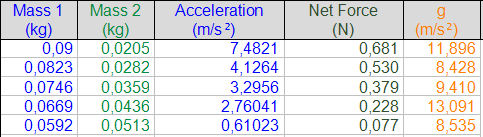
\includegraphics[width=0.5\textwidth]{figures/LoggerPro_bODxuyDhbo.png}
    \caption{Table including \(m_{1}\), \(m_{2}\), \(a\), and the calculated values of \(\Sigma F\) and experimental \(g\)}
    \label{fig:enter-label}
\end{figure}

Using the Logger Pro software, we can keep track of the masses used in each trial and plot the acceleration values recorded in our videos. Acceleration values can be generated from the plot using equation 2, as outlined in the introduction. For example, below is the calculation for the acceleration in the first trial, or \(a_{1}\).

\begin{align}
    \nonumber a_{1}=\frac{2\Delta d}{\Delta t^2} \\
    \nonumber a_{1}=\frac{2(-0.149643))}{(0.2)^2} \\
    \nonumber a_{1}=\frac{-0.299286}{0.04} \\
    \nonumber a_{1}=-7.4821 m/s^2 [up] \\
    \nonumber a_{1}=7.4821 m/s^2 [down]
\end{align}

A column is also calculated for the value of

\begin{equation}
    g(m_{1} - m_{2})
\end{equation}

which represents the net force acting on the system. Further detail will be provided in the next section. For example, here is the net force for the first trial, or \(\Sigma F_{1}\). Unless otherwise stated, the downward direction will be positive. 

\begin{align}
    \nonumber \Sigma F_{1}=g(m_{1} - m_{2}) \\
    \nonumber \Sigma F_{1}=9.8(0.09 - 0.0205) \\
    \nonumber \Sigma F_{1}=0.6811 N [down]
\end{align}

Finally, a column is also calculated for an experimental g value, which will also be discussed in the next section. This information can be seen in figure 1. As an example, below is the calculation for the first experimental g value.

\begin{align}
    \nonumber g_{1} = \frac{a_{1}(m_{1} + m_{2})}{m_{1} - m_{2}} \\
    \nonumber g_{1} = \frac{7.4821(0.09 + 0.0205)}{0.09 - 0.0205} \\
    \nonumber g_{1} = \frac{7.4821(0.1105)}{0.0695} \\
    \nonumber g_{1} = 11.896 m/s^2 [down]
\end{align}

\begin{figure}
    \centering
    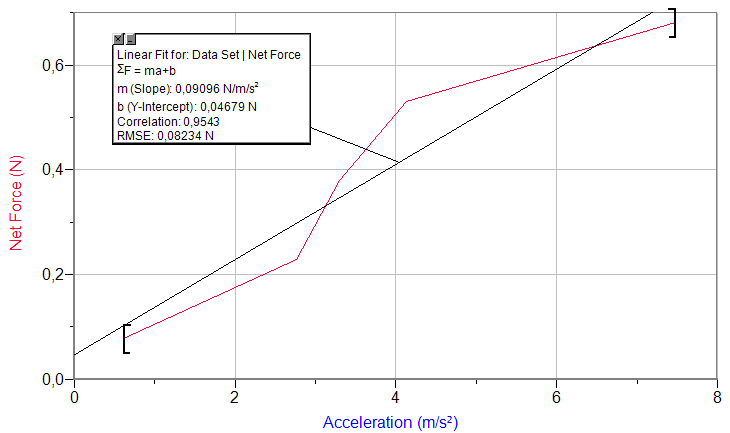
\includegraphics[width=0.5\textwidth]{figures/LoggerPro_BcEtDfO5aS.png}
    \caption{Graph of \(\Sigma F\) over \(a\)}
    \label{fig:enter-label}
\end{figure}

In figure 2, we can observe the graph of the net force over acceleration. After plotting a linear fit over the data, it is evident that as acceleration increases, so does net force. Performing a dimensional analysis shows that the slope of the line is equal to the total mass of the system in \(kg\), since one Newton is equal to a \(\frac{kg\times m}{s^2}\), and acceleration is measured in \(m/s^2\). Evaluating \(\frac{N}{m/s^2}\) shows that the slope should have a value in kilograms, meaning it represents the overall mass of the system. We can also see that m represents the slope by looking at Newton's second law.
The existence of a y intercept which is not equal to 0 is an error, since when the acceleration is zero, the net force should also be zero. 

\section{Discussion Questions}
\subsection{Question One}
\begin{figure}
    \centering
    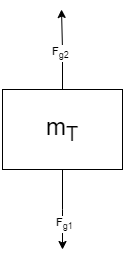
\includegraphics[width=0.2\textwidth]{figures/fbd.drawio.png}
    \caption{Free body diagram demonstrating the forces acting on the system in an Atwood Machine}
    \label{fig:enter-label}
\end{figure}
In figure 3, we can observe the forces acting on the system. The first force is the force of gravity due to mass 1. Assuming that \(m_{1} > m_{2}\), this force of gravity will pull the object downwards towards the centre of the earth. The other force is the force of gravity due to mass 2, which pulls the system in the opposite direction, meaning that when calculating the net force, we subtract the force of gravity due to mass 2 from the force of gravity due to mass 1. Forces of tension are not represented in this free body diagram because they do not have an effect on the net force of the system; both tension forces always pull equally in opposite directions. 
We can derive an expression for the net force by first setting the net force equal to \(F_{g1} - F_{g2}\). This matches what is shown in the figure 3. Then, we can substitute the values of \(g\), \(m_{1}\), and \(m_{2}\), since those are the variables that we have values for. Finally, factor out \(g\).
\begin{align}
    \nonumber \Sigma F = F_{g1} - F_{g2} \\
    \nonumber \Sigma F = gm_{1} - gm_{2} \\
    \nonumber \Sigma F = g(m_{1} - m_{2})
\end{align}
The values generated from this equation can be seen on column 4 of figure 1. 
\subsection{Question Two}
Using the equation found in the last question, we can rearrange it to solve for \(g\).
\begin{align}
    \nonumber \Sigma F = g(m_{1} - m_{2}) = m_{T}a \\
    \nonumber g = \frac{a(m_{1} + m_{2})}{m_{1} - m_{2}}
\end{align}
Using this equation within Logger Pro, we can observe the experimental force of gravity in figure 1. Finding the mean of all experimental \(g\) values gives \(g_{mean} = 10.27 m/s^2\) towards the centre of the Earth.

\begin{align}
    \nonumber g_{mean} = \frac{g_{1} + g_{2} + g_{3} + g_{4} + g_{5}}{5} \\
    \nonumber g_{mean} = \frac{11.896 + 8.428 + 9.410 + 13.091 + 8.535}{5} \\
    \nonumber g_{mean} = 10.27 m/s^2 [down]
\end{align}

Using the following equation, we can find the \(\%_{error}\) of the mean experimental \(g\).

\begin{align}
    \nonumber \%_{error} = 100\frac{|\text{Experimental Value} - \text{Expected Value}|}{\text{Expected Value}} \\
    \nonumber \%_{error} = 100\frac{|10.27-9.8|}{9.8} \\
    \nonumber \%_{error} \approx 4.8\%
\end{align}

This means that the experimental \(g\) value is rather close to the actual \(g\) value. 

\section{Conclusion}
In conclusion, this experiment was a very interesting and valuable way of integrating kinematics with Newton's laws in order to explore movements on an Atwood machine. 
There were likely a few sources of error present. First of all, the floss used as a string in the Atwood machine and the wheel of the pulley may have had forces of friction acting on them. Air resistance may have also played a role in the system. While these forces are extremely small, they can cause a noticeable error in the final results. Additionally, there may have been errors originating from inaccurate mass measurements. Finally, a possible source of error could be due to poor plotting in software, as the plotting in this instance was performed manually. The camera used was also a standard phone camera with a frame rate of approximately 30 frames per second, which made for a blurry video, affecting plotting quality, especially when the masses were in motion.
All of these sources of error culminated in a \(\%_{error}\) of \(\approx 4.8\%\) when calculating an experimental g value. 

\end{document}